
\documentclass[11pt]{article}
\usepackage{acl2014}
\usepackage{times}
\usepackage{url}
\usepackage{subfig}
\usepackage{graphicx}
\usepackage{latexsym}

%\setlength\titlebox{5cm}

\title{Clustering of Co-Occurring Neighboring Unambiguous Terms (COCONUT)}

\author{
Anouk Visser \\
{\tt anouk.visser@student.uva.nl}\\
  \\\And
  R\'emi de Zoeten \\
  {\tt remi.de.z@gmail.com}\\
   \\\And
  Cristina G\^arbacea \\
  {\tt 10407936}
  \\}

\date{}

\begin{document}
\maketitle
\begin{abstract}
Let's decide on the abstract once we finish the body of the text.
  %Vector space models for word representation have shown to be useful in capturing the relationships between words' functions and meanings. Similarities between words are encoded under the form of distance or angle in a high dimensional space. Neural language models, although less used than the traditional \textit{n}-gram models because of their notoriously long training times, present superior performance on the task of word prediction. Leaving from the work of \cite{Mikolov:13}, we propose three new methods for word sense disambiguation based on the co-occurence frequency of the context words near a given target word. We show that these are valid approaches in an unsupervised setting and can increase the accuracy of capturing syntactic and semantic regularities for the English language.
\end{abstract}

\section{Introduction}
Recently \cite{Mikolov:13} found that continuous space word representations capture syntactic and semantic regularities. For example they find that $\textit{queen} - \textit{king} \approx \textit{woman}  -\textit{man}$. The authors use these linguistics regularities to answer a set of analogy questions of the form of `\textit{a} is to \textit{b} as \textit{c} is to \dots'. In this framework, every word is represented by exactly one continuous space word representation. One potential problem when answering analogy questions is that words can be ambiguous. When the analogy is `\textit{seed} is to \textit{apple} as \textit{window} is to \textit{house}' then the word apple refers to a fruit. Another example of an analogy is `\textit{apple} is to \textit{computer} as \textit{porsche} is to \textit{cars}' where the company apple is implied. It is clear that there are words that have two very distinct meanings. By representing words with just one vector (a continuous space representation), as done in \cite{Mikolov:13}, it is not possible to differentiate between the two different meanings of a word. We propose to disambiguate between the various senses of a word in order to obtain multiple continuous space word representations for one word. We will annotate a training corpus to give ambiguous words two different representations. Then we reproduce the steps described in \cite{Mikolov:13} to obtain a continuous space word representation for the different meanings of a word.

We present two different methods for word-sense disambiguation. In section \ref{remi} we describe how word-sense disambiguation can be accomplished by local co-occurrence clustering. In section \ref{anouk} we propose another method, COCONUT, that uses global co-occurrences to disambiguate words.

\section{Related Work}
The linguistic regularities in continuous space word representations used in \cite{Mikolov:13} can be identified by using a vector offset method based on cosine similarity. 

To obtain the continuous space word representations a recurrent neural network language model is used. A Recurrent Neural Networks (RNN) is a neural network that operates in time. At each timestep it accepts an input vector and by the use of nonlinear activation functions it updates its possibly high dimensional hidden state to make a prediction of the output. RNNs are regarded as a rich class model because high dimensional distributed representations can be stored inside their hidden state. In addition, they can implement very complex computations and can perform modelling and prediction tasks for sequences with a highly rich structure.
%XXX The RNN is trained using backpropagation to maximize data likelihood and consists of one input layer that accepts one word at a time encoded using \textit{1}-of-\textit{N} encoding scheme, an output layer which outputs a probability distribution over possible words and a hidden layer with recurrent connections that keeps track of the sentence history.- MAYBE JUST GIVE THE IDEA OF RNNs, INSTEAD OF TELLING THIS. XXX

To answer the question `$a$ is to $b$ as $c$ is to \dots', we use the word vectors $x_a, x_b, x_c$ to determine the word which is assumed to be the best answer to a question. Following the example from the introduction, $\textit{queen} - \textit{king} \approx \textit{woman}  -\textit{man}$, we find that the answer to the question must be $y = x_b - x_a + x_c$. Since it is not likely that $y$ computed in this matter actually exist, we find the answer to the question by maximizing the cosine similarity between y and the words in the corpus. We can also use this method in order to define a similarity between word pairs $a$:$b$ and $c$:$d$. In this case we can answer less obvious analogy questions, we might for example want to find the relationship of competitors as denoted by the word pair \textit{apple}:\textit{dell}. When we are given two new word pairs \textit{china}:\textit{nike} and \textit{ford}:\textit{mercedes} we can rank them by computing the relational similarity: $cos(x_b - x_a + x_c, x_d)$.\\\\
Linguistic regularities can be used in many different unsupervised language learning applications. An example is presented by \cite{MikolovMT:13}, where a method is proposed to exploit similarities among languages for machine translation. For machine translation some sense of a dictionary or phrase table is required. However, these are not always available, or are incomplete. By using two monolingual corpora a model can be trained and linguistic regularities can be learned for the two different languages. If the dictionary entry for \textit{queen} is missing, but, for example, the entry for \textit{king} is available, we can find the translation for \textit{queen} by using the vector offset method as described above.

\section{Word-sense disambiguation by local co-occurrence clustering}
\label{remi}
\begin{figure}
\center
\subfloat[]{
	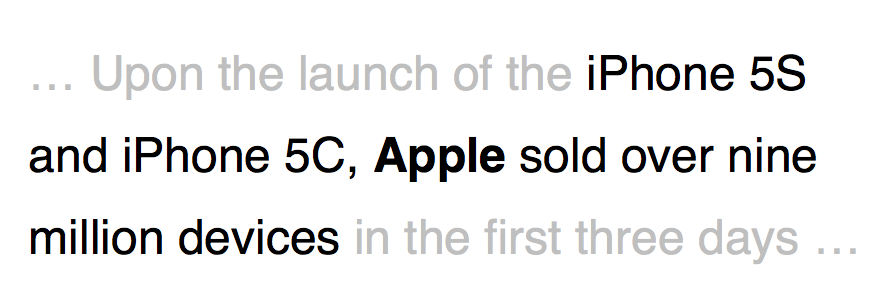
\includegraphics[scale=0.25]{inc.png}
}

\subfloat[]{
	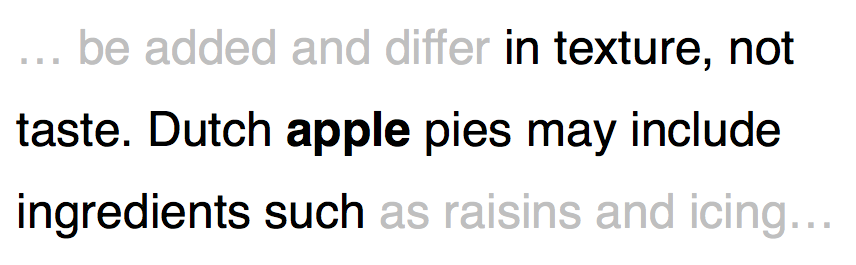
\includegraphics[scale=0.25]{pie.png}
}
\caption{In these two examples for the window around `apple' the black words will be count as co-occurring words, whereas the grey words will be ignored.}
\label{window}
\end{figure}
To find the two senses of a word, one approach would be to cluster different meanings of a word based on the words that it co-occurs with in the corpus. This is done by generating a co-occurrence vector for every time the word is observed in the corpus (this is a local co-occurrence vector). A co-occurrence vector is derived by observing the context of a word. In our experiments the frequency of the words that fall within a window of 5 words from the word that is being observed are encoded into the vector, an illustration can be found in figure \ref{window}. This means that each vector is a sparse vector with the length of the vocabulary size, but can be encoded with at most 10 terms. These co-occurrence vectors are then clustered using k-means clustering. It is possible (even likely) that two co-occurrence vectors do not have a word in common, but still end up in the same cluster. For example, in the case of apple the words \{\textit{technology, iphone, company, revenue}\} might be in the same cluster. Given the co-occurrence vectors, 1:\{\textit{technology, iphone}\}, 2:\{\textit{iphone, revenue}\}, 3:\{\textit{technology, company}\} and 4:\{\textit{company, revenue}\} then 1 and 4 have nothing in common, but can still be bound together by 2 and 3. It should be noted that extracting all co-occurrence vectors from a corpus can require a significant amount of memory, even when using sparse-vector encoding. However, it is possible to have a fine-tunable tradeoff between memory requirements and the number of loops over the corpus (which is more cpu-intensive), by only recording a specific subset of the vocabulary on each iteration.

\section{COCONUT}
\label{anouk}
The COCONUT method for disambiguating words is based on two assumptions: 
\begin{enumerate}
\item the meaning of a word is highly dependent on the words accompanying it
\item the co-occurring words that define one meaning of a word are more likely to co-occur with each other than two words that define two different meanings of the word
\end{enumerate}
In assumption $(1)$ we talk about `words that accompany a word'. In COCONUT, words that accompany a word are co-occurring words. COCONUT will split the co-occurrence vector for \textit{apple} into two co-occurrence vectors, one containing \textit{technology}, \textit{company} and \textit{iPhone}, the other containing \textit{fruit}, \textit{baking} and \textit{pie}. 

An example to further explain assumption (2) can be found in figure \ref{cococ}. Here one meaning of the word \textit{apple} can be characterized by the words \textit{technology}, \textit{company} and \textit{iPhone}, while the other can be characterized by the words \textit{fruit}, \textit{baking} and \textit{pie}. We hypothesize that two words describing one meaning of \textit{apple}, for example, \textit{iPhone} and \textit{technology} are more likely to occur together than two words describing two different meanings, for instance, \textit{iPhone} and \textit{baking}.

Let $C$ be the set of words that co-occur with $A$, the word we want to disambiguate. COCONUT first constructs and converts the global co-occurrence vectors of the words in $C$ to relatedness vectors. It will then cluster these relatedness vectors in order to determine the two possibly different meanings of $A$. 

\begin{figure}
\center
	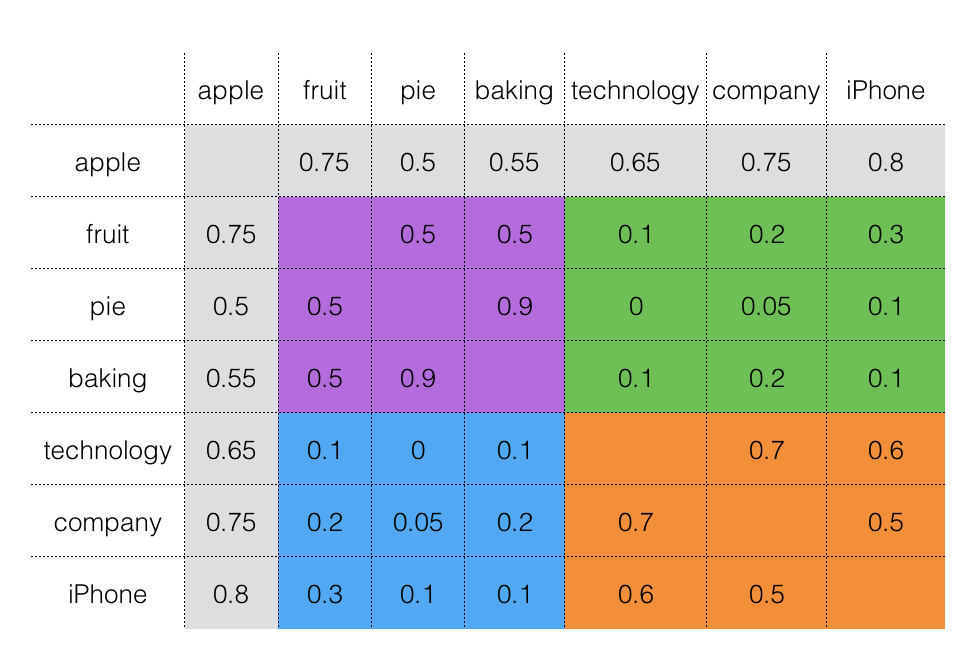
\includegraphics[scale=0.20]{cococ.png}
\caption{Representation of the co-occurrence vectors of the words that co-occur with \textit{apple}. This is just for illustration purposes, neither the co-occurring words or the relatedness scores were obtained from an actual dataset. The grey areas show the co-occurrence vector for the word \textit{apple}. When looking at the co-occurring words, we find that the co-occurring words that describe one meaning of \textit{apple} are more likely to co-occur with each other. The purple area shows that the words \textit{fruit}, \textit{baking} and \textit{pie} are pretty related to each other, whereas they are not so related to \textit{technology}, \textit{company} and \textit{iPhone} (blue area). We observe a similar pattern for the green and orange areas.}
\label{cococ}
\end{figure}

\subsection{Co-Occurrence Vectors}
A global co-occurrence vector contains the frequencies indicating how many times two words co-occur. We obtain the global co-occurrence vector for every word in the corpus in a similar way to how we obtaining the local co-occurrence vector as described in section \ref{remi}. The only difference being that instead of maintaining all local co-occurrence vectors for a given word, we accumulate all local co-occurrence vectors in one global co-occurrence vector. This significantly reduces memory requirements which makes the COCONUT algorithm much more usable. 

After obtaining the global co-occurrence vectors for every word in the corpus, we convert the absolute frequencies in the global co-occurrence vector to a relatedness score. We use the same function for relatedness as \cite{Guthrie:92}:
$$r(x, y) = \frac{f_xy}{f_x+f_y - f_{xy}}$$
where $f_{xy}$ denotes the frequency of $x$ and $y$ occurring together and $f_x$ and $f_y$ denote the frequency of $x$, respectively $y$. 

Words that are not closely related to $A$ do not contribute to either one of the meanings. Therefore, we will discard the words that have a relatedness score with $A$ that falls in the bottom $50\%$ of all relatedness-scores from $C$. The terms that are discarded are considered relevant to all meanings of $A$, we will call this set $R$.

\subsection{Clustering and splitting}
Let the set of co-occurrence vectors from the words in $C$, be called $V$. After applying k-means clustering on the vectors in $V$ we expect to find two cluster centers that represent the two meanings for $A$. Note that we are only interested in describing the two meanings of $A$ using the words in $C$. Therefore, for every vector in $V$ we will discard all words that are not in $C$. The adjusted vectors can now be used to perform k-means clustering. 

The two new co-occurrence vectors for $A$ are initialized with the words in $R$. As the cluster centers define the different meanings of $A$, we can look at the words in each cluster to fill the new co-occurrence vectors for $A$. For example if the words `technology', `iPhone' and `company' are assigned to one cluster, they will be inserted into one of the new co-occurrence vectors for the word `apple' while the words `fruit', `pie', `baking' that were assigned to the other cluster will be inserted into the other co-occurrence vector. 

COCONUT will split every word in the corpus in order to find two different meanings (we excluded the 75 most frequent words), but not all words are ambiguous. We expect that words that have two distinct meanings will have a greater cluster distance (i.e. a greater distance between the two meanings) than words that do not. We discard all disambiguations for the words that have a cluster distance that falls in the bottom $50\%$ of all cluster distances.

\section{Corpus annotation and question answering.}
In our experiments we allowed every word to be split into either one or two different meanings.
Once a set of disambiguated words and their representation has been identified, a new corpus is generated wherein the ambiguous words are annotated with their meaning. This is done by looping over the words in the corpus and again extracting the context of the words that are ambiguous. This context is then matched with either of the clusters that were found for that particular word. We annotate a word with the index of the cluster that best describes its meaning. Then, the process described in \cite{Mikolov:13} is repeated to get the word-vector representation of the words in the annotated corpus. 

Now the question triplet `$a$ is to $b$ as $c$ is to \dots' can be translated into many interpretations, namely `$a\_0$ is to $b\_0 $ as $c\_0 $ is to \dots', `$a\_1$ is to $b\_0 $ as $c\_0 $ is to \dots', etc. If all three words are ambiguous then there are 8 possible interpretations. Of course, not all interpretations are sensible. If the question is `\textit{king} is to \textit{queen} as \textit{man} is to \dots' then the interpretation of \textit{queen} as a band is not sensible, but should be interpreted as `queen as-in royalty'. To achieve this result we first ask the question `which a and which b are most similar?' This is done by combining all senses of \textit{a} and all senses of \textit{b} and measuring their distance. It is assumed that royalty king and royalty queen are closer together than, for example, card-game king and the band queen. We have now reduced the number of questions to only two questions, where \textit{c} is still ambiguous. Now both questions will be answered and an error $\mid\mid \textit{e} \mid\mid$ is determined for each answer, such that $\textit{b} - \textit{a} + \textit{c} \equiv \textit{answer} + \textit{e}$. Finally we choose the answer with the smallest error.

%\section{Latent Semantic Analysis}
%XXX I think this might be better in the related work section, also because we don't have measurements for this method XXX\\
%Unsupervised word sense disambiguation approaches exploit the idea that similar senses of a word have similar neighboring words. They try to induce word senses from input text by clustering word co-occurrences, aiming to divide "the occurrences of a word into a number of classes by determining for any two occurrences whether they belong to the same sense or not" \cite{Schutze:98}.

%\section{Similarity Measures}
%XXX I don't think we should have a section on similarity measures. I think it would be good to mention it in the results section. XXX\\
%Measuring the similarity between two vectors can be seen as an equivalent to measuring their distance. Inversion or subtraction can be easily applied to transform a measure of distance between vectors into a measure of similarity. 

%The most common way to measure similarity between two vectors is to compute the \textit{cosine} of the angle between them as the inner product of the two vectors, after they have been normalized to unit length: $cos(x,y) = \frac{x \cdot y}{||x||\cdot||y||}$. Hence the length of the vectors is irrelevant. \cite{Bullinaria:97} show that the cosine is highly reliable and performs the best, after having compared it with distance measures like Hellinger, Bhattacharya, and Kullback-Leibler. Other common geometric metrics frequently used in the vector space are represented by the Euclidean, Manhattan and Mahalanobis distance, Dice, Jaccard, Pearson and Spearman correlation coefficients.

%The \textit{Euclidean} distance between two points is defined as the length of the line connecting them. In the vector space, it is defined as $d(p,q) = d(q,p) = \sqrt{\sum_{i=1}^{n}(q_i-p_i)^2} $. The smaller this distance the more similar the objects are.  In a similar manner, the \textit{Manhattan} distance is defined as the sum of the absolute differences of the coordinates of two given points as $d(p,q) = |\sum_{i=1}^{n}(p_i - q_i)|$. The \textit{Mahalanobis} distance generalizes the standard Euclidean distance by modelling the relations of elements in different dimensions. Given two vectors $x$ and $y$, their squared Mahalanobis distance is $d_A = (x-y)^T A (x-y)$, where $A$ is a positive semidefinite matrix.

%The \textit{Pearson} correlation coefficient is defined in a similar manner with the Spearman correlation coefficient, with the mention that the last one is between the ranked variables: $\rho=\frac{\sum_i(x_i - \bar{x})(y_i - \bar{y})}{\sqrt{\sum_i(x_i - \bar{x})^2 (y_i - \bar{y})^2 }}$, where $\bar{x} = \frac{\sum_{i=1}^{n}x_i}{n}$ and $\bar{y} = \frac{\sum_{i=1}^{n}y_i}{n}$. A value of 1 indicates total positive correlation, i.e. that a "best fit" line with a positive slope is generated which runs through all the datapoints, a value of 0 means no correlation and a value of -1 represents negative correlation between the two variables. The main advantage of this method over the Euclidean distance is that it is more robust against data which is not normalized.

\section{Evaluation}
We have evaluated the performance of COCONUT on the \textit{enwik8}\footnote{http://cs.fit.edu/~mmahoney/compression/textdata.html} dataset containing a total of 12577300 words and 60237 unique words. 

We performed an empirical evaluating, in which we inspect the two meanings of a word. We also did a quantitative evaluation by using the continuous space word representations to answer a number of analogy questions. Different sets of analogy questions are available. For example the 8000 analogy questions used in \cite{Mikolov:13} contain adjectives (big, bigger, rough, rougher), noun (car, cars, apple, apples) and verb (avoid, avoids, wait, waits) questions. There are also many other analogy questions such as man-woman relations ships, country-currency relationships and more.

\subsection{Similarity Measures}
\begin{figure}
\center
    \begin{tabular}{l|l}
    \textbf{Similarity Metric} & \textbf{Accuracy}  \\ \hline
    Cosine            & 16.20     \\ \hline
    Euclidean         & 16.17     \\ \hline
    Manhattan         & 16.49     \\
    \end{tabular}
    \caption{Results for answering 8000 syntactic analogy questions using the 80-dimensional word projections from \cite{Mikolov:13}}
    \label{sims}

\end{figure}

In \cite{Mikolov:13} the cosine similarity measure is used to find $y$ in $y = b - a + c$. We have tried some other similarity measures or distances to see whether these would improve the accuracy on the set of 800 analogy questions proposed by the authors. Measuring the similarity between two vectors can be seen as an equivalent to measuring their distance. Inversion or subtraction can be easily applied to transform a measure of distance between vectors into a measure of similarity. We report the accuracy for the cosine similarity as well as the euclidean distance and the manhattan distance, using the 80-dimensional word projections from \cite{Mikolov:13} that can be found online\footnote{http://rnnlm.org}. Figure \ref{sims} shows the results for the different similarity measures. Although the manhattan distance slightly outperformed the cosine similarity we have chosen to use cosine similarity because it is not only the most intuitive similarity measure for this problem, but the computation can be performed very efficiently. 

\subsection{Empirical Evaluation}
For the empirical evaluation we have inspected the results of COCONUT on a small hand-made dataset. The hand-made dataset contains different fragments of wikipedia articles on ambiguous topics, it includes apple (fruit, company), queen (band, monarch), jaguar (company, animal), eagles (band, animal), firm (law firm, firm grip), range (of numbers, farm fields) and more. For every ambiguous word we also took fragments from their superclasses. In addition to articles revolving around the ambiguous words, we have also added some random articles.

The results obtained on this small dataset were promising, for example the words from two different clusters  (sorted based on relatedness) for the word `apple' are: 
\begin{enumerate}
\item also, fruit, june, announced, crisp, pie, crumble, inc, 9, is, apples, such, jelly, pomaceous, cake, 77, butter, processor, juice
\item iphone, wwdc, operating, develops, on, x, os, are, 4, sauce, desserts, nokia, remote, towards, offers, system, largest, worlds
\end{enumerate}
Another example is `jaguar' for which we find: 
\begin{enumerate}
\item feline, fords, under, dropped, solitary, enjoys, waters, threatened, preferred, sustained, inland, 59, rainforest, swimming, across, ownership, largely, exceptionally, planned
\item models, sported, has, plated, traditionally, chrome, prominently, forming, famous, changed, hunts, grounds, associated, featured, americas, fishing
\end{enumerate}
There is a fair amount of noise in the different clusters, but overall there is a reasonably clear distinction between the two different meanings of these words.
On the \textit{enwik8} dataset we find a lot more noise in the two clusters, including a lot of words that are relevant to both clusters. When inspecting the clusters we noticed that the words with the highest relatedness to the disambiguated word were most likely to be correct. However, the majority of the words that show little relatedness (XXXXX even if they are in the top $50\%$ of related words) do not describe the meaning as well. We provide two more examples of clusters formed on the \textit{enwik8} dataset:\\\\
`santa'
\begin{enumerate}
\item claus, maria', monica, clara, tenerife, ana, san, croce, christmas
\item cruz, fe, barbara, catarina, grande, california, marta, mar, del
\end{enumerate}
We observe a lot of noise in this example. However, the meaning of `santa'-as-in Christmas is captured in meaning 1, whereas the meaning of `santa'-as-in location is captured in meaning 2. \\\\
`belief'
\begin{enumerate}
\item god, faith, knowledge, justification, jesus, religion, absence, afterlife, resurrection
\item contrary, justified, atheism, systems, deities, beliefs, lack, freedom, feminism
\end{enumerate}
Meaning 1 is more centered around `belief'-as-in religion, whereas meaning 2 is more centered around a multitude of beliefs. 

\subsection{Quantitative Evaluation}
\section{Future work}
\subsection{Co-occurrence vectors}
would also be possible to use a soft-max or gaussian measure to weigh each word based on its distance, but we have weighted each of the 10 words in the 5 word window equally.
\subsection{Detecting ambiguousness}
One of the most challenging problems in word-sense disambiguation is deciding whether a word is ambiguous or not. At this point we discard all disambiguations that have a cluster distance that fall in the bottom $50\%$. In order to gain more insight in the distribution of these cluster distance we have made some plots. From these plots we see that most of the words are concentrated around a cluster distance of approximately 0.9. We do find that there are many words that have a cluster distance below 0.9 as well, in total this were X unique words, that together make up X$\%$ of the corpus. In future work, we might want to focus on finding a better way of detecting whether a word is ambiguous or not. 
\subsection{Detecting number of meanings}
In our work we only split the words, i.e. we assume that a word can have at most two meanings. This is not a very solid assumption, we find many difference meanings including 1) financial institute 2) land alongside a river 3) cushion of a pool table. While inspecting the clusters, we found a lot of words that we would not consider ambiguous might occur in many different contexts, slightly changing the meaning of a word. An example of a word that we found has many different meanings is `red'. This word had so many different meanings, that two word senses were not enough, we provide a limited breakdown of the words that co-occur with `red':
\begin{itemize}
\item Boston Red Sox - sports
\item Red Sea, Red Square - places
\item Communism, love - concepts
\item Relief, Red Cross - non-profits / brands
\item \dots
\end{itemize} 
We believe that splitting the word vector for `red' should still boost the performance when answering analogy questions. The analogy question `\textit{red} is to \textit{sox} as \textit{blue} is to \dots' might be difficult to answer when all different meanings of the word `red' are encoded into one word representation. Once we are able to disambiguate the word `red' we find a word representation that is focused at sports and not so much at communism. (the answer to `\textit{red} is to \textit{sox} as \textit{blue} is to \dots' is `jays' as in Toronto Blue Jays, another question we could ask is `\textit{red} is to \textit{boston} as \textit{blue} is to \dots') In future work we should not restrict ourselves to a fixed number of meanings of one word, but investigate ways to determine how many meanings a word actually has. 
 
\section{Conclusion}
\begin{thebibliography}{}

\bibitem[\protect\citename{Mikolov \bgroup et al.\egroup }2013a]{Mikolov:13}
Tomas Mikolov, Wen-tau Yih, and Geoffrey Zweig.
\newblock 2013a.
\newblock Linguistic regularities in continuous space word representations.
\newblock Proceedings of NAACL-HLT, 
746--751

\bibitem[\protect\citename{Mikolov \bgroup et al.\egroup }2013b]{MikolovMT:13}
Tomas Mikolov, Quoc V. Le and Ilya Sutskever.
\newblock 2013b.
\newblock Exploiting Similarities among Languages for Machine Translation.
\newblock arXiv preprint arXiv:1309.4168, 

\bibitem[\protect\citename{Guthrie \bgroup et al.\egroup }1991]{Guthrie:92}
Joe A. Guthrie, Louise Guthrie, Yorick Wilks and Homa Aidinejad.
\newblock 1991.
\newblock Subject-dependent co-occurrence and word sense disambiguation.
\newblock Proceedings of the 29th annual meeting on Association for Computational Linguistics, 
146--152
\newblock
Association for Computational Linguistics

\bibitem[\protect\citename{Bullinaria \bgroup et al.\egroup }1997]{Bullinaria:97}
John Bullinaria and John Levy.
\newblock 1997.
\newblock Extracting semantic representations from word co-occurrence statistics: A computational study.
\newblock Behaviour Research Methods, 
510--526

\bibitem[\protect\citename{Schutze \bgroup et al.\egroup }1998]{Schutze:98}
Schutze H.
\newblock 1998.
\newblock Automatic Word Sense Discrimination.
\newblock Computational Linguistic, 
97

\bibitem[\protect\citename{Martens \bgroup et al.\egroup }2011]{Martens:13}
Martens James and Ilya Sutskever
\newblock 2011.
\newblock Learning Recurrent Neural Networks with Hessian-Free Optimization.
\newblock Proceedings of the 28th International Conference on Machine Learning

\end{thebibliography}

\end{document}
